% 第3章第5节：波动方程与能量传播（初值解与传播速度；能量估计与解的稳定性）。

\section{波动方程与能量传播}
\label{sec:pde-wave}

热方程中曲率决定变化的速度，波动方程中曲率决定变化的加速度。多出的这一阶时间导数让场具有惯性：它会越过平衡位置，把扰动以有限速度传向远处，并且不会自行停下来。本节先在全直线和区间上求出解，看清传播与反射；再用能量估计证明唯一性和连续依赖，并与热方程的耗散对照。

\subsection{初值解与传播速度}
\label{sec:pde-wave-solution}

\paragraph{弦的振动方程}
设一根弦沿$x$轴绷紧，张力为$T$，线密度为$\rho$，$u(x,t)$是它在$x$处的竖直位移。取一小段$[a,b]$，两端的张力沿弦的切线方向，竖直分量约为$T\sin\theta\approx T\tan\theta=Tu_x$，这里用了小斜率近似。净竖直力为$T\bigl(u_x(b,t)-u_x(a,t)\bigr)=\int_a^bTu_{xx}\,\mathrm dx$。由Newton第二定律，它等于这一段的质量乘加速度$\int_a^b\rho u_{tt}\,\mathrm dx$。区间任意，得到\term{波动方程}（wave equation）
\begin{equation}
  u_{tt}=c^2u_{xx},\qquad c=\sqrt{T/\rho} .
  \label{eq:pde-wave-1d}
\end{equation}
推导忽略了弦的水平运动、重力与空气阻力，并假设斜率很小。在$d$维中，膜的振动与声波满足$u_{tt}=c^2\Delta u$。

方程对时间是二阶的，所以需要两个初值：初位移$u(x,0)=u_0(x)$与初速度$u_t(x,0)=u_1(x)$。这与上一章的二阶常微分方程$\ddot x=-\omega^2x$需要初始位置和速度是同一回事；更准确地说，场的状态是一对函数$(u,u_t)$，而不只是位移。

\paragraph{d'Alembert公式}
在整条实轴上，方程可以完全解出。对$C^2$函数，混合偏导数可交换，于是$u_{tt}-c^2u_{xx}=(\partial_t-c\partial_x)(\partial_t+c\partial_x)u$：波动算子是两个一阶输运算子的乘积，一个向右、一个向左。引入特征坐标$\xi=x-ct$、$\eta=x+ct$，方程变为$u_{\xi\eta}=0$，所以$u_\xi$与$\eta$无关，积分两次得$u=F(\xi)+G(\eta)$：解是一个右行波与一个左行波之和。

用初值确定$F$与$G$：$F+G=u_0$，$-cF'+cG'=u_1$。后者积分得$G-F=c^{-1}\int_0^xu_1+K$，与前者联立解出$F,G$，代回得
\begin{equation}
  u(x,t)=\frac12\bigl[u_0(x-ct)+u_0(x+ct)\bigr]+\frac1{2c}\int_{x-ct}^{x+ct}u_1(s)\,\mathrm ds .
  \label{eq:pde-dalembert}
\end{equation}
这就是\term{d'Alembert公式}（d'Alembert's formula）。若$u_0\in C^2(\mathbb R)$、$u_1\in C^1(\mathbb R)$，可以直接验证它是$C^2$解：$t=0$时第一项为$u_0$、第二项为零；对$t$求导再令$t=0$，第一项给出$\tfrac12[-cu_0'+cu_0']=0$，第二项给出$\tfrac1{2c}[cu_1(x)+cu_1(x)]=u_1(x)$。上面的推导又说明每个$C^2$解都具有这一形式，所以解唯一。

初速度为零时，初始形状分成两半，各以速度$c$向左右跑开，形状不变。图~\ref{fig:pde-dalembert}(a)画出了这一过程：$t=0.75$时两半还有重叠，之后完全分开，各自的高度都是原来的一半。

\begin{figure}[!htb]
  \centering
  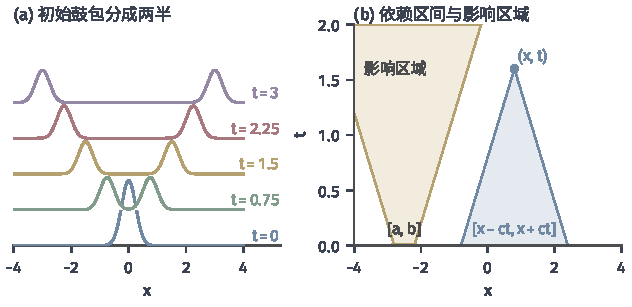
\includegraphics[width=107mm]{figures/03-optimization-evolution-and-signals/02-processes-and-trajectory-evolution/matplotlib/pde-dalembert/figure.pdf}
  \caption{全直线上的波动方程，$c=1$。(a)~初位移$u_0=e^{-(x/0.35)^2}$、初速度为零的d'Alembert解在五个时刻的形状，竖直方向错开排列：鼓包分成两个半高的行波。(b)~$(x,t)$平面中的依赖与影响：点$(x,t)$的值只依赖初始数据在蓝色三角形底边$[x-ct,x+ct]$上的值；支撑在$[a,b]$上的初始数据只影响黄色区域$[a-ct,b+ct]$。}
  \label{fig:pde-dalembert}
\end{figure}

\paragraph{有限传播速度}
式~\eqref{eq:pde-dalembert}显示，点$(x,t)$处的值只依赖$u_0$在两点$x\pm ct$处的值和$u_1$在区间$[x-ct,x+ct]$上的值。这个区间称为点$(x,t)$的\term{依赖区域}（domain of dependence）。反过来，若初始数据在$[a,b]$外为零，那么在时刻$t$，解在$[a-ct,b+ct]$外为零，扰动只影响这个以速度$c$扩张的\term{影响区域}（domain of influence）。图~\ref{fig:pde-dalembert}(b)画出了这两个区域：信号以有限速度$c$传播。

热方程完全不同。在全直线上，可以直接验证热核
\[
  \Phi(x,t)=\frac1{\sqrt{4\pi\kappa t}}\exp\Bigl(-\frac{x^2}{4\kappa t}\Bigr),\qquad t>0
\]
满足$\Phi_t=\kappa\Phi_{xx}$：两边都等于$\Phi\cdot\bigl(-\tfrac1{2t}+\tfrac{x^2}{4\kappa t^2}\bigr)$。对有界连续的初值，$u(x,t)=\int\Phi(x-y,t)u_0(y)\,\mathrm dy$给出热方程的解，图~\ref{fig:pde-three-mechanisms}(a)中Gauss鼓包方差增大$2\kappa t$正是这个卷积的结果。由于$\Phi$处处为正，只要$u_0\geq0$且不恒为零，任意$t>0$时$u(x,t)$在所有$x$处都为正：一点的加热瞬间被无穷远处感知到。热方程的传播速度是无穷大，这是扩散模型在极小尺度上的理想化。

\paragraph{有界区间：反射与驻波}
把弦的两端固定在$x=0$与$x=1$，$u(0,t)=u(1,t)=0$。一种求解办法是镜像：把$u_0,u_1$关于$x=0$作奇延拓、再延拓成周期为$2$的函数，对延拓后的数据用d'Alembert公式。延拓后的数据关于$x=0$与$x=1$都是奇的，解也保持这种奇性，所以两端恒为零。物理上，一个脉冲跑到固定端后被翻转方向反射回来，就像从镜子里出来一个倒影的脉冲。

另一种办法是找保持形状的解。仿照热方程的模式，设$u=a(t)\sin(k\pi x)$，代入得$a''=-(k\pi c)^2a$，所以
\[
  u(x,t)=\sin(k\pi x)\bigl[A\cos(k\pi ct)+B\sin(k\pi ct)\bigr] .
\]
这是\term{驻波}（standing wave）：形状固定，整体以角频率$\omega_k=k\pi c$上下振荡，在$x=j/k$处的节点永远不动。与热方程的模式相比，同样的空间形状对应的时间因子从$e^{-k^2\pi^2t}$变成了$\cos(k\pi ct)$：前者衰减，后者永远振荡。图~\ref{fig:pde-standing-waves}画出了前三个模式；边界条件决定了允许的波长只能是$2/k$。

\begin{figure}[!htb]
  \centering
  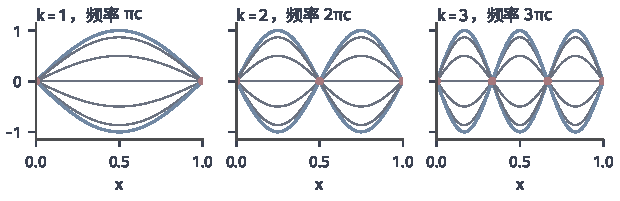
\includegraphics[width=105mm]{figures/03-optimization-evolution-and-signals/02-processes-and-trajectory-evolution/matplotlib/pde-standing-waves/figure.pdf}
  \caption{两端固定的弦的前三个驻波$\sin(k\pi x)\cos(k\pi ct)$。每幅图叠画了$k\pi ct=0,\pi/6,\ldots,\pi$七个时刻的形状，蓝色为最大位移；红点为节点$x=j/k$。模式不衰减，第$k$个模式的角频率为$k\pi c$。}
  \label{fig:pde-standing-waves}
\end{figure}

一般初值用$e_k=\sqrt2\sin(k\pi x)$展开：记$a_k=\langle u_0,e_k\rangle$、$b_k=\langle u_1,e_k\rangle$，
\begin{equation}
  u(t)=\sum_{k=1}^\infty\Bigl[a_k\cos(\omega_kt)+\frac{b_k}{\omega_k}\sin(\omega_kt)\Bigr]e_k .
  \label{eq:pde-wave-series}
\end{equation}
它在什么意义下是解，取决于初值的光滑程度。若$u_0\in H_0^1(0,1)$、$u_1\in L^2(0,1)$，则$\sum_kk^2\pi^2a_k^2=\|u_0'\|^2<\infty$（分部积分给出$\langle u_0',\sqrt2\cos(k\pi x)\rangle=k\pi a_k$，而$u_0'$的均值为零，再用余弦系的完备性与Parseval等式），$\sum b_k^2=\|u_1\|^2<\infty$，于是级数在$H_0^1$中、它的时间导数在$L^2$中关于$t$一致收敛；这是下一小节能量空间中的解。要得到经典解，需要系数衰减得更快，例如$\sum k^2|a_k|<\infty$与$\sum k|b_k|<\infty$可以保证逐项求两阶导数后一致收敛。

与热方程的定理~\ref{thm:pde-heat-series}对照，这里没有任何因子帮助级数收敛：$\cos(\omega_kt)$不衰减，初值有多粗糙，解在所有时刻就有多粗糙。拨弦时初始形状是三角形$u_0=\min(x,1-x)$，$a_k=2\sqrt2\sin(k\pi/2)/(k^2\pi^2)$只按$k^{-2}$衰减，$\sum k^2|a_k|$发散；三角形的尖角不会被磨平，而是分成两个折点，以速度$c$来回跑动、在两端反射，永远存在。形式上写出级数，不等于得到了经典解。

\subsection{能量估计与解的稳定性}
\label{sec:pde-wave-energy}

\paragraph{动能与势能}
弦的能量由两部分组成：动能$\tfrac12\int\rho u_t^2$与拉伸储存的弹性势能，后者在小斜率近似下为$\tfrac12\int Tu_x^2$。除以$\rho$，对$\Omega\subset\mathbb R^d$上的$u_{tt}=c^2\Delta u+f$定义
\begin{equation}
  E(t)=\frac12\int_\Omega\bigl(u_t^2+c^2|\nabla u|^2\bigr)\,\mathrm d\bm x .
  \label{eq:pde-wave-energy}
\end{equation}
设$u$足够光滑。对$t$求导，并对含$\nabla u\cdot\nabla u_t$的项用Green恒等式~\eqref{eq:pde-green-identity}，
\[
  E'(t)=\int_\Omega u_t\bigl(u_{tt}-c^2\Delta u\bigr)\,\mathrm d\bm x+c^2\int_{\partial\Omega}u_t\,\partial_{\bm n}u\,\mathrm dS
  =\int_\Omega fu_t\,\mathrm d\bm x+c^2\int_{\partial\Omega}u_t\,\partial_{\bm n}u\,\mathrm dS .
\]
边界项在两种常见条件下都消失：固定端$u=0$对所有$t$成立，所以边界上$u_t=0$；自由端$\partial_{\bm n}u=0$。于是无源时$E'(t)=0$，能量守恒：动能与势能来回转换，总量不变。

有源时，$E'=\langle f,u_t\rangle\leq\|f\|\,\|u_t\|\leq\|f\|\sqrt{2E}$。为了避免在$E=0$处除以零，对$\varepsilon>0$考察$\sqrt{E+\varepsilon}$：
\[
  \frac{\mathrm d}{\mathrm dt}\sqrt{E+\varepsilon}=\frac{E'}{2\sqrt{E+\varepsilon}}\leq\frac{\|f\|\sqrt{2E}}{2\sqrt{E+\varepsilon}}\leq\frac{\|f\|}{\sqrt2},
\]
积分后令$\varepsilon\to0$，得
\begin{equation}
  \sqrt{E(t)}\leq\sqrt{E(0)}+\frac1{\sqrt2}\int_0^t\|f(s)\|\,\mathrm ds .
  \label{eq:pde-wave-energy-source}
\end{equation}
源项注入的能量随时间累积，但不会被放大。

\paragraph{唯一性与连续依赖}
设$u_1,u_2$是同一问题的两个光滑解，差$w$满足无源方程、零初值与齐次边界条件。$w$的能量在$t=0$为零，又守恒，所以恒为零，于是$w_t=0$、$\nabla w=0$，$w$是常数；它的初值为零，所以$w\equiv0$。对数据不同的两个解，把式~\eqref{eq:pde-wave-energy-source}用于差，得到能量范数下的连续依赖：初位移的梯度、初速度和源项的小扰动，只引起位移梯度与速度的小变化。

这一估计也指出了波动方程自然的状态空间：位移属于$H_0^1$（或相应边界条件下的$H^1$），速度属于$L^2$，即$(u,u_t)\in H_0^1\times L^2$，能量正是这个乘积空间中的范数平方（差一个常数）。在这个空间中，可以仿照第~\ref{sec:pde-heat-semigroup}小节用Galerkin逼近定义并构造弱解，式~\eqref{eq:pde-wave-series}在$u_0\in H_0^1$、$u_1\in L^2$下给出的就是它。还要注意，把$t$换成$-t$，波动方程不变：由时刻$T$的位移和速度反推初值，与正向求解一样适定，这与反向热方程的严重不适定形成对照。

\paragraph{阻尼与耗散}
若弦在空气中振动，受到与速度成正比的阻力，方程变为$u_{tt}+\gamma u_t=c^2u_{xx}$，$\gamma>0$。同样的计算给出$E'=-\gamma\|u_t\|^2\leq0$，能量递减。逐个模式看，振幅满足$a''+\gamma a'+\omega_k^2a=0$；$\omega_k>\gamma/2$时振幅按$e^{-\gamma t/2}$衰减，能量大约按$e^{-\gamma t}$衰减，并带有动能与势能交替带来的起伏。

图~\ref{fig:pde-energy-compare}比较了三种情形的能量。无阻尼的波动能量是一条水平线；阻尼波动的能量沿$e^{-0.5t}$阶梯式下降，在速度为零的时刻（能量全部为势能）阻尼暂时不做功；热方程的能量单调衰减。

\begin{figure}[!htb]
  \centering
  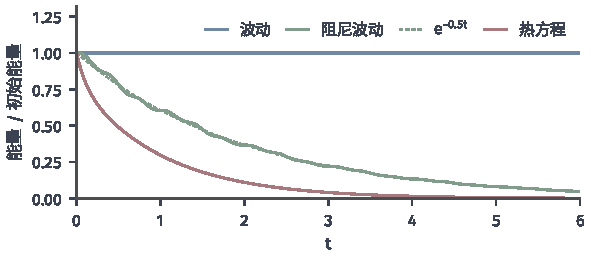
\includegraphics[width=100mm]{figures/03-optimization-evolution-and-signals/02-processes-and-trajectory-evolution/matplotlib/pde-energy-compare/figure.pdf}
  \caption{区间$(0,1)$上两端为零、初值$\sin(\pi x)+\tfrac12\sin(3\pi x)$的三种演化的能量，均相对初始能量归一化。波动方程$u_{tt}=u_{xx}$（初速度为零）的能量$\tfrac12\int(u_t^2+u_x^2)$守恒；阻尼波动$u_{tt}+0.5u_t=u_{xx}$的能量沿虚线$e^{-0.5t}$下降；热方程$u_t=0.05u_{xx}$的能量$\tfrac12\int u^2$单调衰减。曲线由精确的模式解计算。}
  \label{fig:pde-energy-compare}
\end{figure}

两种衰减的来源不同。热方程对时间是一阶的，能量等式~\eqref{eq:pde-heat-energy}中自动出现$-\|\nabla u\|^2$，耗散是方程结构本身带来的，不需要额外的项。无阻尼波动方程的能量等式中没有这样的项，能量严格守恒；衰减只能来自外加的阻尼。所以热方程的耗散结论、磨光效应与最大值原理都不能搬到波动方程上。最大值原理的失效有一个简单的例子：全直线上取$u_0=0$、$u_1\geq0$为一个非零鼓包，初始位移处处为零，由式~\eqref{eq:pde-dalembert}，$t>0$时在鼓包附近$u>0$，最大值并不在初始时刻取到。
